\documentclass[11pt,a4paper]{article}
\usepackage{tikz}
\usetikzlibrary{arrows.meta,positioning}
\usepackage{tabularx}
\usepackage{amsmath,amssymb,amsthm}
\usepackage{geometry}
\geometry{margin=1in}
\usepackage{hyperref}
\usepackage{graphicx}
\usepackage{setspace}
\onehalfspacing

\title{\textbf{Paper C-03: Trade Networks:\\ A Constraint-Driven Flux Dynamics (CDFD) Perspective}}
\author{Steve Bico Mujjabi, MD\\
\small Independent Researcher\\
\small Founder, Vura Labs\\
\small Kampala, Uganda\\
\small ORCID: 0009-0001-0556-5516}
\date{August 2026}

\begin{document}
\maketitle

% BEGIN SHARED-METHODS POINTER
\noindent\textit{Shared Part IV notation and evidence boundaries are defined in \path{PART_IV_METHODS_AND_CLAIM_BOUNDARY.md}. This paper states only its local observables, comparison, and failure conditions.}
% END SHARED-METHODS POINTER


\begin{abstract}
This paper develops a falsifiable CDFD/AFL model of Trade Networks. It maps goods, services, capital, information, and contractual demand to driving flux $\Phi$, ports, tariffs, logistics, finance, and network dependencies to active constraint $C$, substitution, inventory, rerouting, diplomacy, and production change to responsiveness $S$, and contracts, specialization, infrastructure, and disruption history to structural memory $M_s$. The target outcome is trade volume, shortages, prices, and recovery, tested against customs data, input-output tables, shipping traces, prices, and disruption records. The paper treats universality as a shared model architecture rather than an assertion that unlike systems have the same material mechanism. It states the negative result that would make the mapping unnecessary and places the domain claim inside the cumulative CDFD programme and its reproducible runtime boundary.
\end{abstract}

\section{Introduction}

The global economy is a singular, highly integrated fluid network. Capital, technology, and raw materials naturally seek to flow from regions of surplus to regions of deficit, driven by the thermodynamic gradient of profit and necessity.

However, nations frequently intervene in this natural flow for geopolitical reasons. Tariffs, embargoes, and sanctions act as artificial dams placed across the river of global commerce. In CDFD, a sovereign state implementing a tariff is actively manipulating the topological constraints of the global active surface.

\section{The Geoeconomic Adaptive Surface}
We govern bilateral and global trade using the Adaptive Operating Ratio:
\begin{equation}
    \Psi_s = \left( \frac{\Phi}{C} \right) \cdot S \cdot M_s
\end{equation}

For a specific trade corridor between two nations:
\begin{itemize}
    \item \textbf{Flux ($\Phi$)}: The monetary value and physical volume of exports and imports crossing the border.
    \item \textbf{Constraint ($C$)}: Tariffs, quotas, regulatory misalignment, and outright economic sanctions.
    \item \textbf{Responsiveness ($S$)}: The elasticity of the domestic economy to substitute imports, find alternative trading partners, or pivot domestic production.
    \item \textbf{Memory ($M_s$)}: Decades-long trade agreements, entrenched supply chains, and specialized infrastructure (e.g., specific pipelines or localized shipping hubs). High memory locks the economy into dependency on a specific partner.
\end{itemize}

\subsection{Trade Wars and Topological Severing}
In a free-trade era, tariffs are low, and $\Phi$ is extremely high. The global system is highly integrated and operates in a sustained growth regime ($\Psi_s > 1$).

If a trade war begins, nation A applies a massive tariff against nation B. The constraint $C$ spikes artificially. If nation B's economy is highly specialized and dependent on this specific corridor (high memory $M_s$), it cannot easily pivot. The adaptive ratio for that specific trade sector crashes to $\Psi_s \ll 1$.

The flow $\Phi$ of critical components ceases. The sanctioned or tariffed nation enters an ischemic economic state. To survive, the nation must drastically increase its internal responsiveness $S$---forcing expensive domestic production or forging entirely new, inefficient trade corridors with secondary nations. The artificial constraint forces a massive, thermodynamically inefficient topological rewiring of the global surface.



\section{Measurement Layer}

% BEGIN PART IV MAJOR CROSS-DOMAIN UPGRADE
\section{Cross-Domain Model Upgrade: Mechanism, Scale, and Tests}

\subsection{Observable Translation}

The paper-specific translation begins with an observable chain rather than a
verbal analogy. For Trade Networks, the proposed drive is goods, services, capital, information, and contractual demand.
The active limitation is ports, tariffs, logistics, finance, and network dependencies. Responsiveness is carried by
substitution, inventory, rerouting, diplomacy, and production change, while retained state is represented by
contracts, specialization, infrastructure, and disruption history. The outcome to explain is trade volume, shortages, prices, and recovery.

\begin{table}[htbp]
\centering
\small
\caption{Operational CDFD/AFL map for Paper C-03.}
\begin{tabularx}{\textwidth}{|l|X|X|}
\hline
\textbf{Term} & \textbf{Paper-specific observable meaning} & \textbf{Measurement question} \\
\hline
$\Phi$ & goods, services, capital, information, and contractual demand & What rate, load, gradient, or demand enters the focal system? \\
\hline
$C$ & ports, tariffs, logistics, finance, and network dependencies & Which measured bottleneck limits transfer, function, or recovery? \\
\hline
$S$ & substitution, inventory, rerouting, diplomacy, and production change & Which process changes effective capacity or reroutes the load? \\
\hline
$M_s$ & contracts, specialization, infrastructure, and disruption history & Which retained state makes equal present loads produce different futures? \\
\hline
$Y$ & trade volume, shortages, prices, and recovery & Which outcome is predicted out of sample, with uncertainty? \\
\hline
\end{tabularx}
\end{table}

\begin{figure}[htbp]
\centering
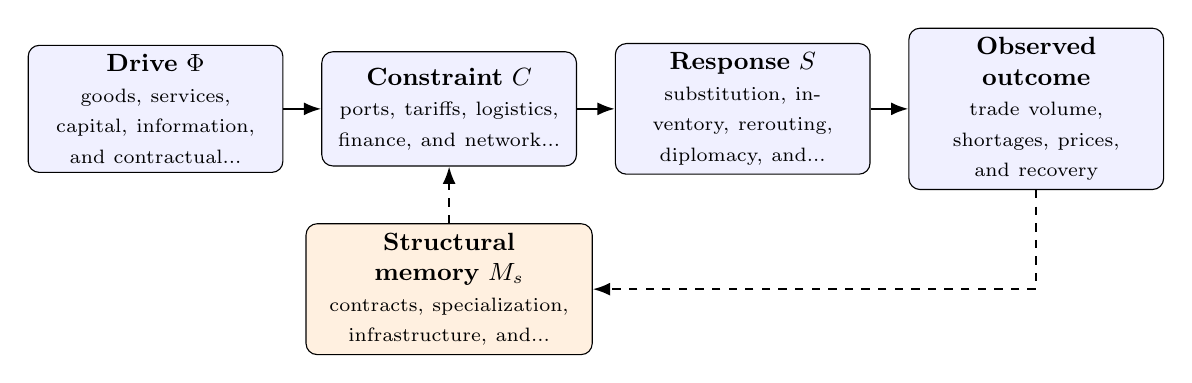
\begin{tikzpicture}[
    node distance=0.48cm,
    every node/.style={font=\small},
    box/.style={draw, rounded corners, align=center, minimum height=1.45cm, text width=3.0cm, fill=blue!6},
    memory/.style={draw, rounded corners, align=center, minimum height=1.25cm, text width=3.4cm, fill=orange!12},
    flow/.style={-{Latex[length=2.2mm]}, thick},
    feedback/.style={-{Latex[length=2.2mm]}, thick, dashed}
]
\node[box] (drive) {\textbf{Drive $\Phi$}\\\scriptsize goods, services, capital, information, and contractual...};
\node[box, right=of drive] (constraint) {\textbf{Constraint $C$}\\\scriptsize ports, tariffs, logistics, finance, and network...};
\node[box, right=of constraint] (response) {\textbf{Response $S$}\\\scriptsize substitution, inventory, rerouting, diplomacy, and...};
\node[box, right=of response] (outcome) {\textbf{Observed outcome}\\\scriptsize trade volume, shortages, prices, and recovery};
\node[memory, below=0.72cm of constraint] (memory) {\textbf{Structural memory $M_s$}\\\scriptsize contracts, specialization, infrastructure, and...};
\draw[flow] (drive) -- (constraint);
\draw[flow] (constraint) -- (response);
\draw[flow] (response) -- (outcome);
\draw[feedback] (outcome.south) |- (memory.east);
\draw[feedback] (memory.north) -- (constraint.south);
\end{tikzpicture}
\caption{Paper C-03 observable CDFD/AFL architecture for Trade Networks. Solid arrows give the proposed forward chain; dashed arrows make history-dependent feedback explicit.}
\label{fig:c03-architecture}
\end{figure}

\subsection{Paper-Specific Causal Hypothesis}

For this paper, the hypothesized causal sequence is specific. A change in
goods, services, capital, information, and contractual demand arrives faster than substitution, inventory, rerouting, diplomacy, and production change can compensate.
This raises or redistributes ports, tariffs, logistics, finance, and network dependencies. If the load persists,
the retained state encoded by contracts, specialization, infrastructure, and disruption history changes the next response, so a later event of equal
magnitude can produce a different trajectory in trade volume, shortages, prices, and recovery. The
scientific task is to estimate that sequence against the best ordinary model of
the domain, not merely to redescribe the outcome after it occurs.

\subsection{Cross-Scale Translation Without Mechanistic Erasure}

For the socioeconomic systems family, the cross-domain translation compares human and institutional throughput, unequal access to capacity, adaptive coordination, and historical path dependence. The variables are not morally neutral: aggregation can hide who receives flow, who bears constraint, and whose prior losses become persistent memory. \cite{BarabasiAlbert1999,WattsStrogatz1998,Holling1973,Shannon1948}
The required scale declaration for this paper is days to decades; firms to the world economy. At short
scales, the key question is whether the incoming drive is transmitted,
buffered, or diverted. At intermediate scales, response changes effective
capacity and network exposure. At long scales, retained structure can alter the
state space itself. A result is genuinely cross-scale only when the aggregation
rule is stated and the same conclusion is not an artifact of averaging.

\subsection{Evidence Ladder and Discriminating Tests}

\begin{table}[htbp]
\centering
\small
\caption{Evidence ladder for Paper C-03. Each rung can fail independently.}
\begin{tabularx}{\textwidth}{|p{0.17\textwidth}|X|X|}
\hline
\textbf{Test} & \textbf{Design} & \textbf{Discriminating result} \\
\hline
Proxy audit & Measure customs data, input-output tables, shipping traces, prices, and disruption records and preregister how each record maps to $\Phi$, $C$, $S$, $M_s$, and $Y$. & The mapping fails if proxies are non-identifiable, circular, or change meaning across cases. \\
\hline
Load ramp & Apply or observe a corridor closure or supplier loss during high demand while estimating the dominant constraint and response time. & A threshold claim requires a reproducible nonlinear change and uncertainty bounds, not a visually chosen breakpoint. \\
\hline
Recovery and memory & Match present load across units with different histories, then compare recovery paths. & The memory claim requires history-dependent divergence after current conditions are controlled. \\
\hline
Model comparison & Compare the baseline domain model with and without the CDFD/AFL state variables using held-out data. & The paper's stated falsifier is: network memory does not improve shortage or trade-recovery prediction. \\
\hline
\end{tabularx}
\end{table}

\subsection{Research Programme and Boundary Conditions}

The immediate research programme has four steps. First, construct a documented
dataset from customs data, input-output tables, shipping traces, prices, and disruption records and retain raw units before normalization.
Second, fit a baseline domain model and report its calibration and out-of-sample
error. Third, add the smallest identifiable CDFD/AFL state extension and test
whether it improves prediction of trade volume, shortages, prices, and recovery. Fourth, repeat the
analysis across the declared scale range and publish negative cases as part of
the cross-domain translation audit.

% END PART IV MAJOR CROSS-DOMAIN UPGRADE

\section{Conclusion}
Trade wars and sanctions are not merely political tools; they are the intentional weaponization of thermodynamic constraints. By framing international trade within CDFD, we see that global commerce behaves as an adaptive biological membrane. Artificial geopolitical constraints force traumatic structural adaptations, supporting the testable hypothesis that economic isolation can drive either violent internal restructuring or systemic decay.
\section*{Conflict of Interest} The author declares no conflict of interest.
\section*{Data Availability}
Part-specific runtime diagnostics are under each Part's \path{outputs/} directory.

Release-wide code: \path{Part_E_Synthesis/supplementary/}.

Generated summaries: \path{Part_E_Synthesis/outputs/}.

Figures: \path{Part_E_Synthesis/figures/}.


\section{Reference Layer}
\bibliographystyle{plain}
\bibliography{universal_afl_references}
\end{document}
